% !TEX TS-program = pdflatex
% !TEX encoding = UTF-8 Unicode

% This is a simple template for a LaTeX document using the "article" class.
% See "book", "report", "letter" for other types of document.

\documentclass[11pt]{article} % use larger type; default would be 10pt


\usepackage{ulem}
\newcommand\NoIndent[1]{%
  \par\vbox{\parbox[t]{\linewidth}{#1}}%
}


\usepackage[utf8]{inputenc} % set input encoding (not needed with XeLaTeX)

%%% Examples of Article customizations
% These packages are optional, depending whether you want the features they provide.
% See the LaTeX Companion or other references for full information.

%%% PAGE DIMENSIONS
\usepackage{geometry} % to change the page dimensions
\geometry{a4paper} % or letterpaper (US) or a5paper or....
% \geometry{margin=2in} % for example, change the margins to 2 inches all round
% \geometry{landscape} % set up the page for landscape
%   read geometry.pdf for detailed page layout information

\usepackage{graphicx} % support the \includegraphics command and options

% \usepackage[parfill]{parskip} % Activate to begin paragraphs with an empty line rather than an indent

%%% PACKAGES
\usepackage{booktabs} % for much better looking tables
\usepackage{array} % for better arrays (eg matrices) in maths
\usepackage{paralist} % very flexible & customisable lists (eg. enumerate/itemize, etc.)
\usepackage{verbatim} % adds environment for commenting out blocks of text & for better verbatim
\usepackage{subfig} % make it possible to include more than one captioned figure/table in a single float
% These packages are all incorporated in the memoir class to one degree or another...

%%% HEADERS & FOOTERS
\usepackage{fancyhdr} % This should be set AFTER setting up the page geometry
\pagestyle{fancy} % options: empty , plain , fancy
\renewcommand{\headrulewidth}{0pt} % customise the layout...
\lhead{}\chead{}\rhead{}
\lfoot{}\cfoot{\thepage}\rfoot{}

%%% SECTION TITLE APPEARANCE
\usepackage{sectsty}
\allsectionsfont{\sffamily\mdseries\upshape} % (See the fntguide.pdf for font help)
% (This matches ConTeXt defaults)

%%% ToC (table of contents) APPEARANCE
\usepackage[nottoc,notlof,notlot]{tocbibind} % Put the bibliography in the ToC
\usepackage[titles,subfigure]{tocloft} % Alter the style of the Table of Contents
\renewcommand{\cftsecfont}{\rmfamily\mdseries\upshape}
\renewcommand{\cftsecpagefont}{\rmfamily\mdseries\upshape} % No bold!

%%% END Article customizations


\usepackage{verbatim}
\usepackage{amsmath}


\title{Work Log for November 10th-14th}
\author{Logan Brown}
%\date{} % Activate to display a given date or no date (if empty),
         % otherwise the current date is printed 

\begin{document}
\maketitle
%\tableofcontents


\section{Goals for the Week}
%Paste output from writeWeek
\begin{enumerate}
	\item RC example
	\item Load external R packages, use them with RC
\end{enumerate}

\section{Progress/Notes}

\subsection{RC example}

The RC example calculates the line of best fit for the collatz length of 1 to 1000. Here's how the output will typically look

\begin{verbatim}
[lbrown@star1 RC]$ make exec
../../EXTLIB/MPICH/mpich-shared/bin/mpirun -n 1 ./driver RCcar.cfg
Initializing the executive...
rank 0 going to statically run 'RC'
Executing --file=script.r
Line of Best Fit: y=0.0322921x + 44.3798
Standard Deviation = 40.87291
Graph written to CollatzGraph.pdf 
Data written to CollatzData.csv 
\end{verbatim}

And here's CollatzGraph.pdf.

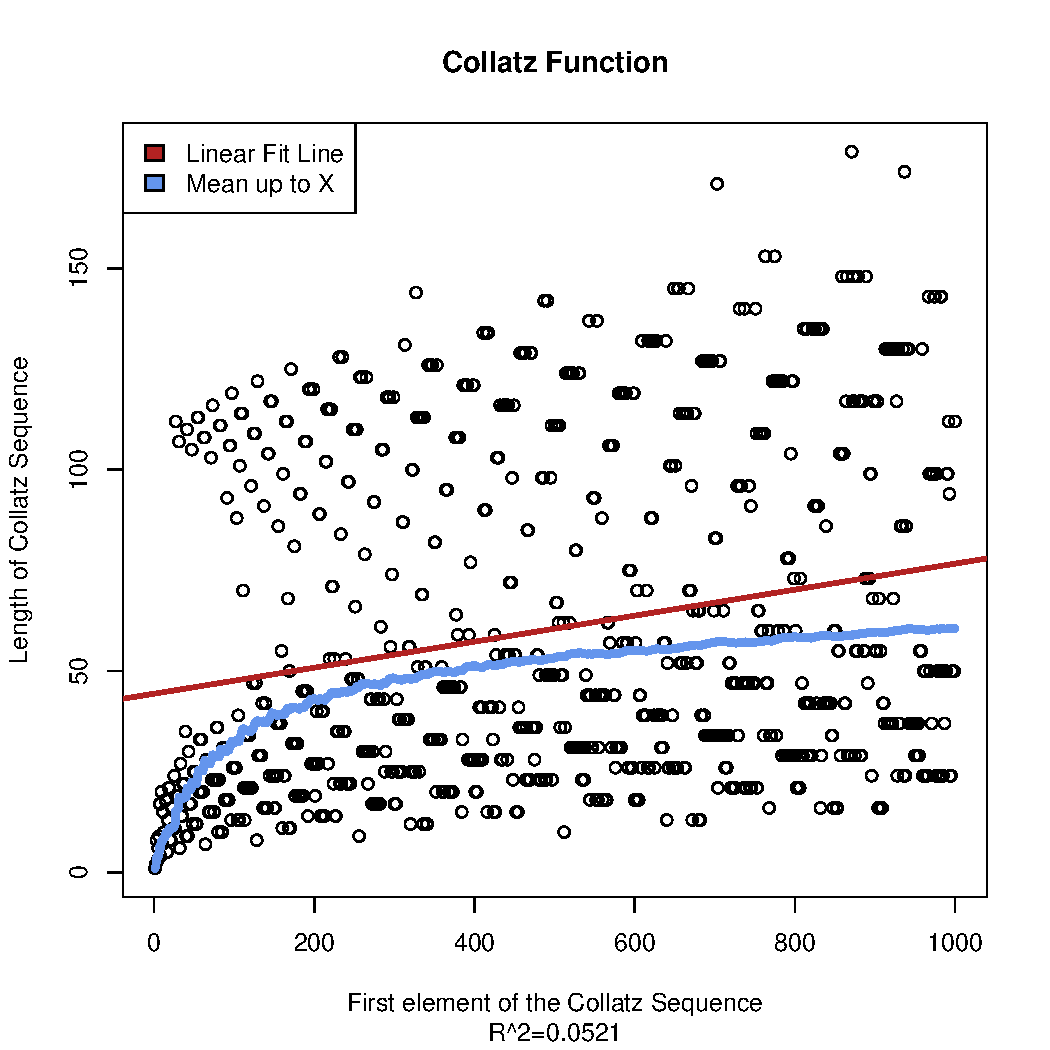
\includepdf[pages={1}]{data/CollatzGraph.pdf}

\subsection{Load external R packages, use them with RC}


\subsection{Documentation}

\subsubsection{Document the RC car}
Just comment the code

Added in a section at the beginning describing the code. 
\begin{verbatim}
/********************************************************************
 * Written by Logan Brown
 * NICS and UTK, 2014
 *
 * This code defines an IEL module function that executes 'script.r'
 * using the R language interpreter. Script.r must be placed in the
 * directory where the driver code is executed.
 *
 * iel-2.0/CASES/RC has an example using the Collatz Conjecture
 *
********************************************************************/
\end{verbatim}

And added a similar section to the R script
\begin{verbatim}
############################################################################
# Script written by Logan Brown
# NICS and UT Knoxville, 2014
# This script finds the length the sequences generated by the following rule
#
#    Let a_0 be an integer. For all n > 0
#       a_(n+1) = (a_n)/2        if a_n is even; 
#       a_(n+1) = 3(a_n) + 1     if a_n is odd and a_n != 1
#    When a_n = 1 the sequence stops (otherwise it cycles 1, 4, 2, 1, 4...)
#
# The script finds the length of these sequences for the first 1000 inputs
# by default, with the number of inputs determined by "number". It then
# finds a line of best fit for the increasing sequence length, and gets
# the standard deviation of the sequence lengths.
# It also writes out the calculated data to a file, and generates a graph.
############################################################################
\end{verbatim}




\subsubsection{Ising Model}
Write up a paragraph on the Ising Model -- Done. See Ising.pdf

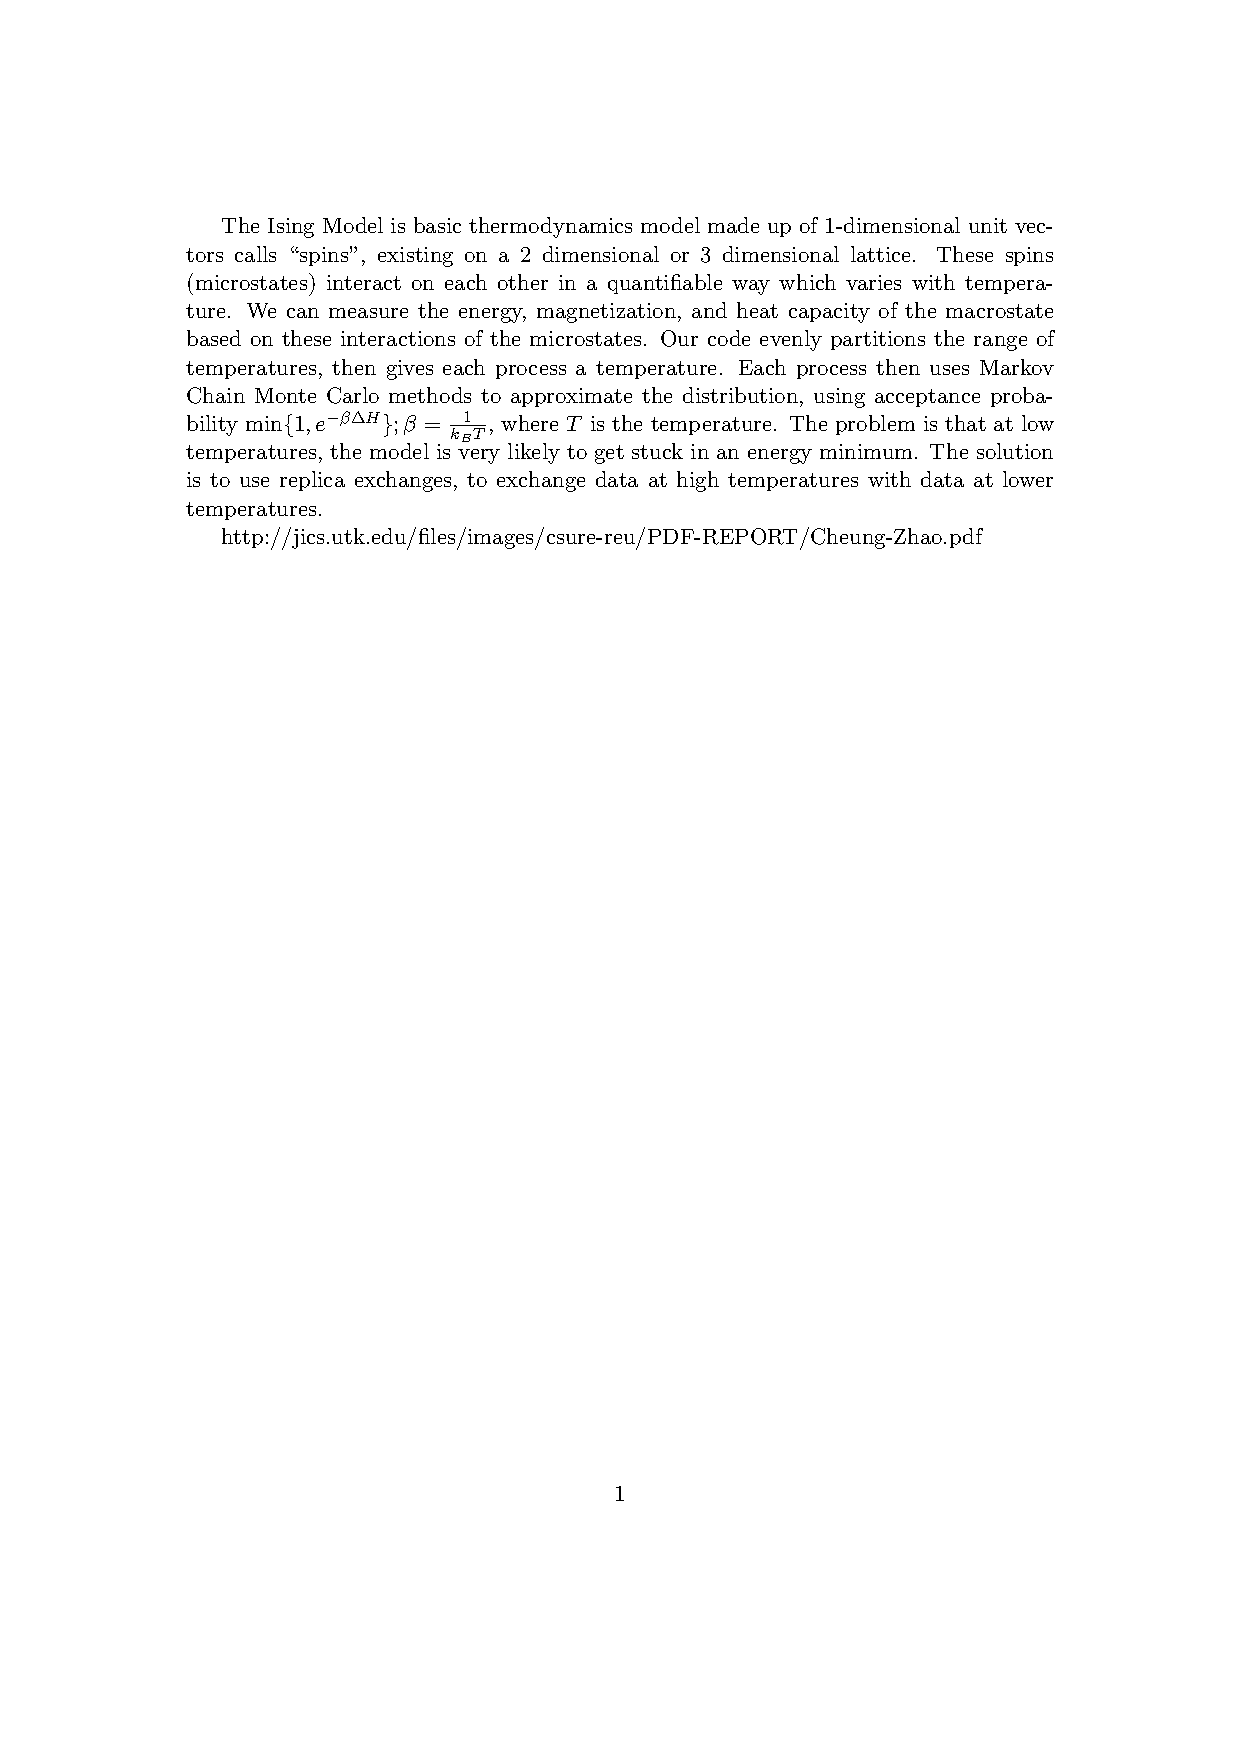
\includepdf[pages={1}]{ising.pdf}

\subsection{Read through paper for Kwai}

I made some notes. Do we want to talk about Kraken? 

\section{Goals for next Week}
\begin{enumerate}
\item PSUADE
\item DAKOTA
\item Further documentation?
\end{enumerate}


\end{document} %End of day document, REMOVE
